\section*{4/6/2562}

เนื่องจากเข้าทำงานเป็นวันแรก จึงต้องจัดสถานที่ทำงาน และทำงานต่อจากที่ได้รับมอบหมายก่อนการฝึกงาน

งานที่ได้รับมอบหมายโดยคร่าวคือการวิเคราะห์สภาวะความง่วงในคน โดยศึกษาจากกลุ่มเป้าหมายของพนักงานบริษัท
ซึ่งอาจารย์ที่ปรึกษาให้สิทธิ์ในการกำหนดแนวทางการวิเคราะห์ได้โดยอิสระ อย่างไรก็ตามงานของการวิเคราะห์ความง่วง
โดยตั้งต้นนั้นมักใช้การวิเคราะห์ภาพจากดวงตา (gaze monitoring) ซึ่งใช้วันนี้ในการหางานวิจัยตั้งต้น

นอกจากนี้ยังศึกษาแนวทาง ข้อกำหนด และมาตรฐานจริยธรรมในการทดลองภายในมนุษย์ (human subject research)

\section*{5/6/2562}

ศึกษาแนวทางในการทำ eye gazing ตามหนังสือที่ได้รับมอบหมาย และนำเสนองานวิจัยต่อจากที่เลือกจากเมื่อวาน

ปรับแก้แนวทางในการวิจัย และได้รับมอบหมายให้ออกแบบวิธีการทดลองโดยคร่าว
หารือกับทีมโปรแกรมเมอร์ว่าด้วยซอฟต์แวร์สำหรับการทดลอง

\section*{6/6/2562}

ศึกษาอุปกรณ์สำหรับติดตามดวงตา (Gazepoint) ก่อนจะพบว่าอุปกรณ์มีข้อจำกัดในการทำงานบางส่วน ทำให้ไม่สามารถดึง
ภาพดวงตาออกมาใช้ในโปรแกรมภายนอกได้ และติดต่อกับผู้ผลิตอุปกรณ์เพื่อหารือความเป็นไปได้ในการดึงภาพดวงตา

ศึกษาการใช้ Pytorch ในการทำการเรียนรู้เชิงลึก (deep learning) แทนที่ Keras

\section*{7/6/2562}

เปลี่ยนแนวทางการทำวิจัยด้วยข้อจำกัดของอุปกรณ์ มาเป็นการทำวิจัยบนกล้ามเนื้อตา (EOG) ค้นคว้าและทบทวนวรรรณกรรม
ที่เกี่ยวข้องกับงาน

ทำแบบทดสอบสำหรับบทเรียนจริยธรรมการวิจัยในมนุษย์จนอยู่ในเกณฑ์ได้รับประกาศนียบัตรผ่านการอบรม

\section*{10/6/2562}

นักเรียนจากโครงการพัฒนาอัจฉริยภาพทางวิทยาศาสตร์เข้ามาร่วมในทีม โดยการทดลองในส่วนของ Drowsiness research
ถูกแบ่งออกเป็นสองงานที่ต้องทดลองร่วมกัน จึงต้องตกลงแนวทางการทดลองให้ชัดเจน

ทดลองให้นักเรียนดังกล่าวศึกษาการวัดคลื่นสมองโดยอุปกรณ์ OpenBCI, ให้คำแนะนำถึงการเตรียมผิวหนัง (skin preparation)
ก่อนการติดอิเล็กโทรด, การเลือกใช้ชนิดอิเล็กโทรดและข้อดี-ข้อเสียของอิเล็กโทรดแต่ละชนิด

\section*{11/6/2562}

ทำงานที่ได้รับมอบหมายต่อจากเมื่อวาน

\section*{12/6/2562}

นัดประชุมงานกับอาจารย์ที่ปรึกษาโครงการ สรุปแนวทางการทดลอง และตัดสินใจเพิ่มการวัด PVT (Psychomotor vigilance task)
เพิ่มเติมในการทดลอง

เขียนโปรแกรมสำหรับทดสอบ PVT โดยใช้การสื่อสารบนอุปกรณ์หลายเครื่องเพื่อลดความจำเป็นในการซื้อปุ่ม (physical button)
ด้วยเหตุผลทางงบประมาณ

ช่วงเย็นรับประทานอาหารเย็นร่วมกับอาจารย์ธงชัย ชิวปรีชา

\section*{13/6/2562}

ได้รับมอบหมายให้ทดลองจับภาพตาเพื่อหา PERCLOS ด้วยกล้องเว็บแคมแบบที่มีหลอดอินฟราเรด ในเบื้องต้นสามารถครอปตัดเฉพาะส่วน
ที่เป็นลูกตาออกจากภาพใบหน้าแบบเต็มหน้าได้ อย่างไรก็ตาม ไม่ประสบความสำเร็จในการคำนวนร้อยละพื้นที่ของตาดำที่ไม่ถูกหนังตาบดบัง

\begin{figure}[H]
    \centering
    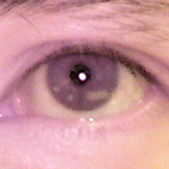
\includegraphics[width=0.4\textwidth]{images/268.png}
    \caption{ภาพถ่ายตาจากล้อง IR}
\end{figure}